\section{Concluding remarks}
\label{sec:concluding-remarks}

\begin{figure}[t]
\centering
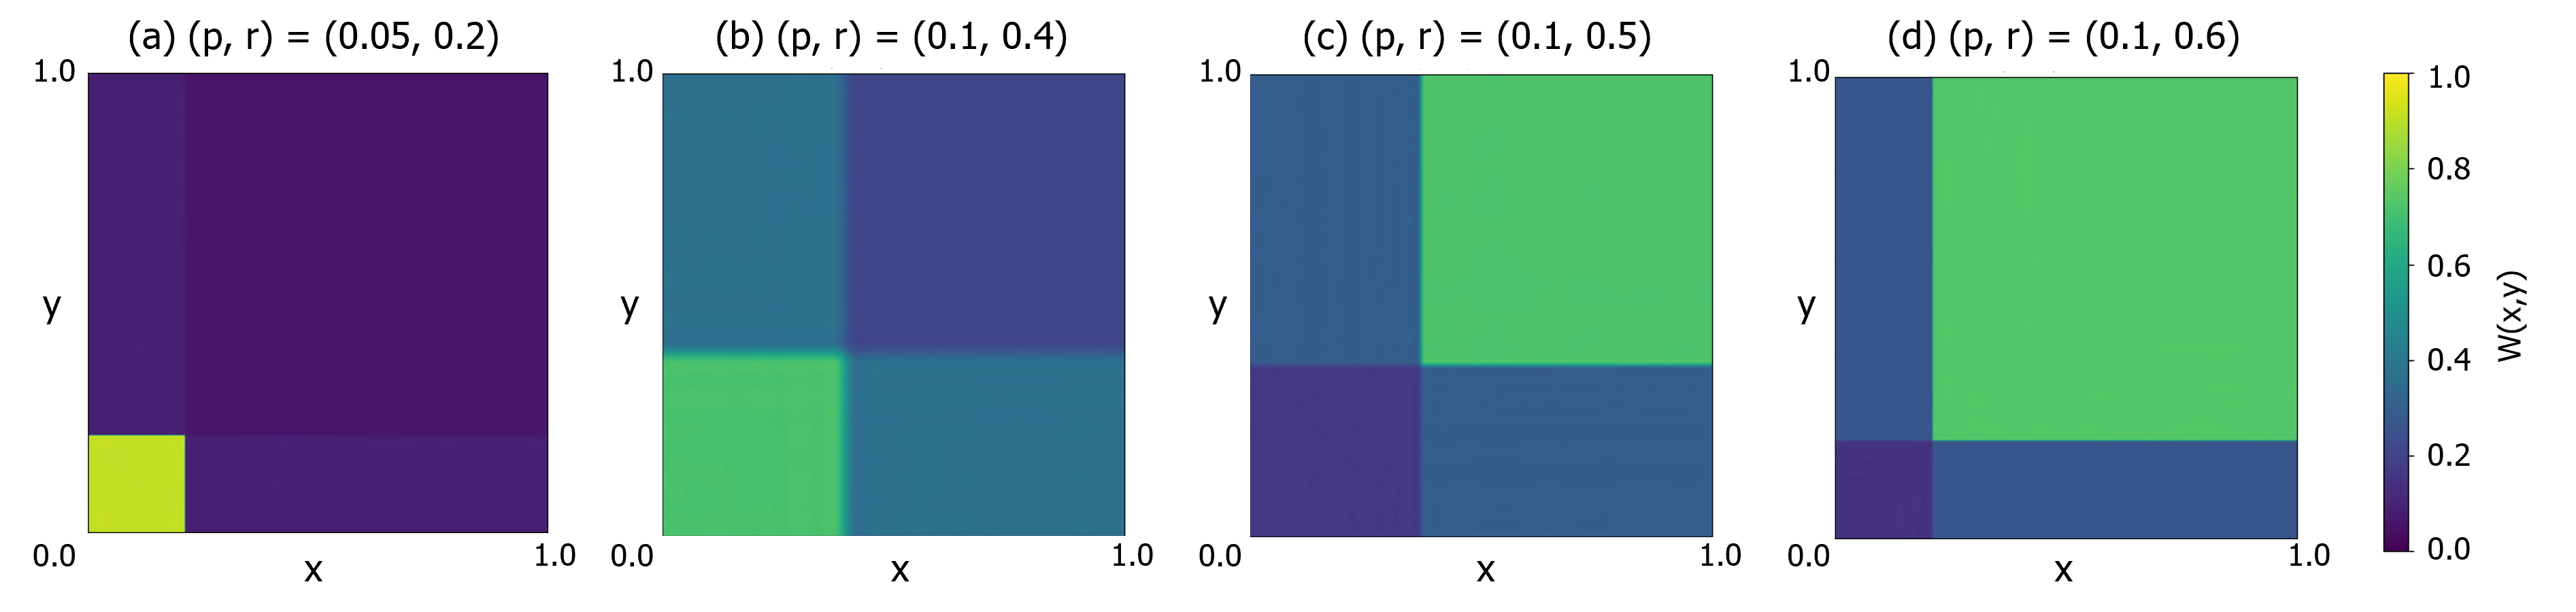
\includegraphics[width=\textwidth]{figures/neural_graphon_representation.png}
\caption{Graphons learned for $H=K_3$ by optimizing
\eqref{eq:graphon-variational-problem} using the neural representation of
Kim, Baek, Lee, and Yang~\cite{KimBaekLeeYangGraphons}.
Each heatmap shows $W(x,y)$ for the indicated parameter pair $(p,r)$ in the symmetry-breaking region;
colour denotes edge probability.  The two-block patterns support an
affirmative answer to the bipodality question.}
\label{fig:neural-bipodal-patterns}
\end{figure}

In this paper, we analyze the structure of the optimizers of
the Chatterjee--Varadhan variational problem for regular graphs.
More precisely, \Cref{thm:nonexceptional-optimizers} establishes the uniqueness
and bipodal structure of the nonconstant optimizers in a small neighbourhood of
the Lubetzky--Zhao boundary except at the exceptional density $r_*=(d-1)/d$.
\Cref{thm:endpoint-optimizers} constructs an analytic curve approaching
the boundary point $(\pc(r_*),r_*)$ at this exceptional density.
Along this curve, the unique optimizers are rank-one and bipodal, and
both block sizes tend to $1/2$.  This differs from the vanishing-block
behaviour as $p\uparrow\pc(r)$ at a fixed nonexceptional density~$r$.

A natural question is whether the bipodality and uniqueness established in
\Cref{thm:nonexceptional-optimizers,thm:endpoint-optimizers} persist throughout
the symmetry-breaking region.
For $H=K_3$, the numerical experiments in \Cref{fig:neural-bipodal-patterns}
suggest that bipodality persists throughout this region.
Assuming bipodality, the experiments in \Cref{fig:bipodal-parameter-maps}
explore how the two within-block edge densities, the cross-block edge density,
and the size $\alpha$ of the block with the higher within-block density vary
with $(p,r)$.
These computations suggest a curve along which uniqueness fails and across
which some of the bipodal parameters change discontinuously.
Such discontinuities would prevent an analytic continuation of the bipodal
parameters throughout the region, even if the optimizers remain bipodal.
Understanding the optimizers throughout this region and resolving the
bipodality question raised by Lubetzky and
Zhao~\cite[Section~7]{lubetzky2015large} would therefore require methods that can
accommodate possible nonuniqueness and discontinuous changes in the
parameters.

\begin{figure}[t]
\centering
\begin{tikzpicture}
\node[anchor=south west,inner sep=0] (parameterplots) at (0,0)
  {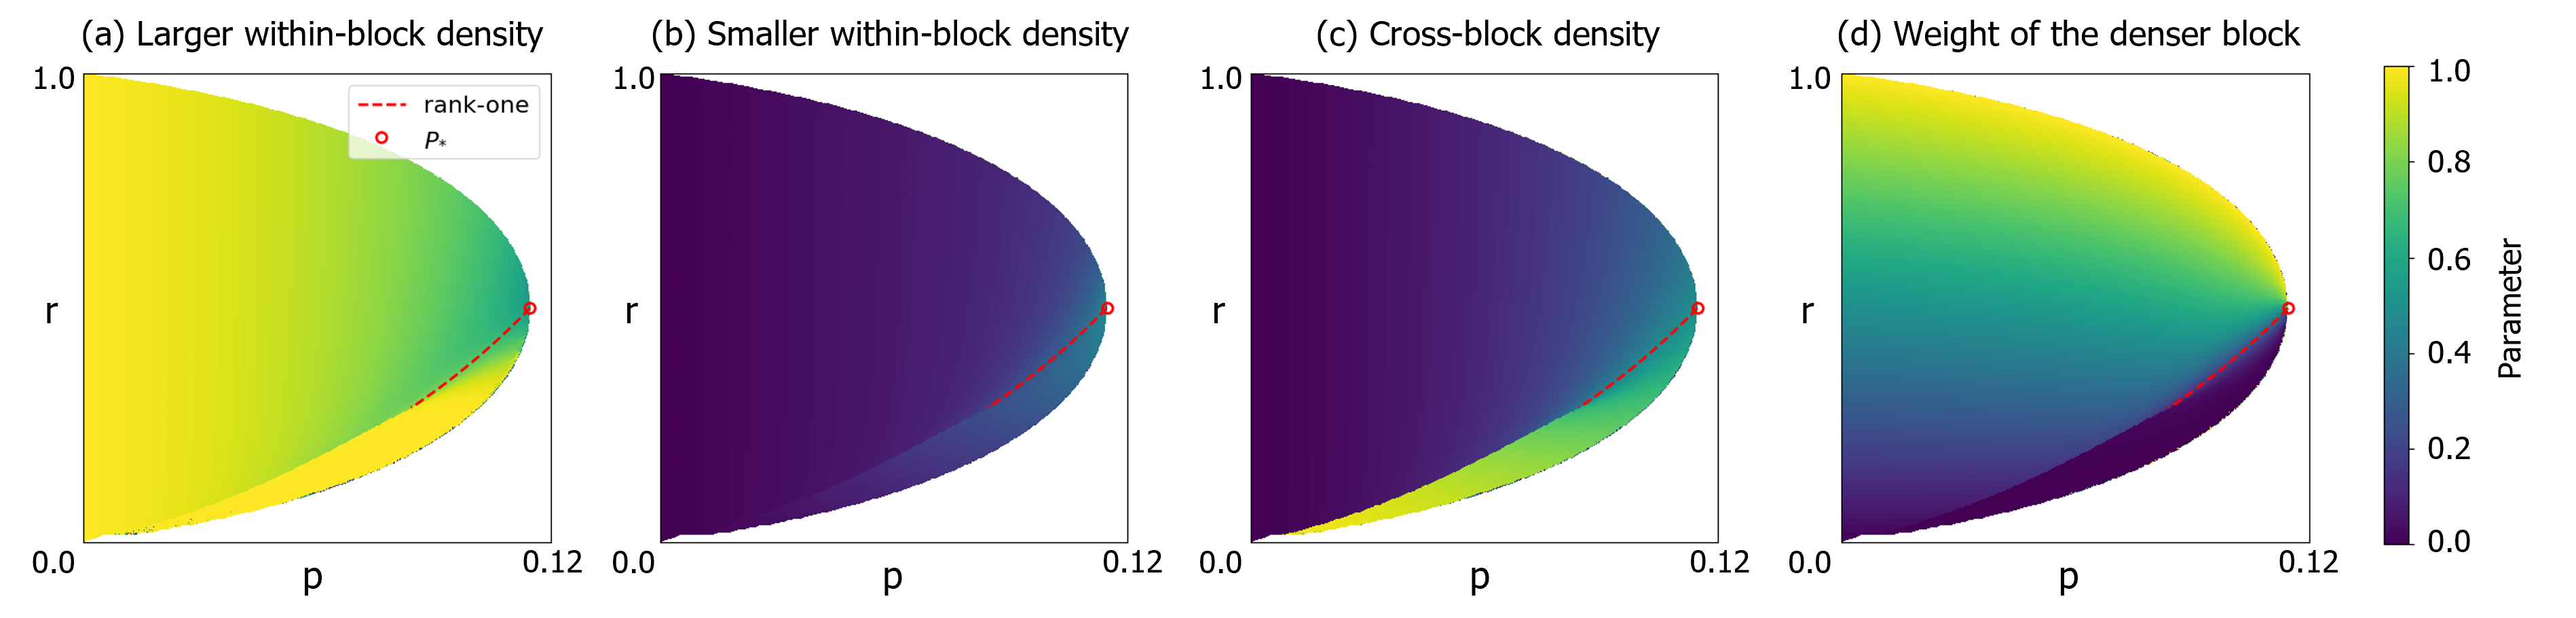
\includegraphics[width=\textwidth]{figures/numerical_optimization.png}};
% Typeset the panel titles here so their terminology follows the manuscript.
\begin{scope}[x={(parameterplots.south east)},y={(parameterplots.north west)}]
  \fill[white] (0.02,0.90) rectangle (0.90,1);
  \node[font=\sffamily\fontsize{6}{7}\selectfont] at (0.122,0.955)
    {(a) Higher within-block density};
  \node[font=\sffamily\fontsize{6}{7}\selectfont] at (0.349,0.955)
    {(b) Lower within-block density};
  \node[font=\sffamily\fontsize{6}{7}\selectfont] at (0.575,0.955)
    {(c) Cross-block density};
  \node[font=\sffamily\fontsize{6}{7}\selectfont] at (0.802,0.955)
    {(d) Size of the denser block};
\end{scope}
\end{tikzpicture}
\caption{Numerically optimized bipodal parameters for $H=K_3$ in the
symmetry-breaking region.  Panels (a)--(d) show, respectively, the higher
and lower of the two within-block edge densities, the cross-block edge
density, and the size $\alpha$ of the block with the higher within-block
edge density.  Here $\alpha$ is the Lebesgue measure of that block and
can be greater or less than $1/2$: the denser block need not be the larger
block.
The dashed red curve traces the interior near-rank-one parameters approaching $P_*$
(red circle).  This observation motivated the rank-one bipodal family constructed
in \Cref{sec:rank-one-stationary-family}.}
\label{fig:bipodal-parameter-maps}
\end{figure}

Our numerical observations for $H=K_3$ suggest the following conjecture for
general regular graphs.  Its final assertion extends the $\alpha_*=1/2$ case proved
in \Cref{thm:endpoint-optimizers} to arbitrary limiting smaller-block
sizes $\alpha_*\in(0,1/2]$.
\begin{conj}
\label{conj:symmetry-breaking-optimizers}
Let $H$ be a $d$-regular graph with $d\ge2$, and write
$\mathcal B_H:=\{(p,r)\in(0,1)^2:p<\pc(r)\}$ for the symmetry-breaking region.
The optimizers of \eqref{eq:graphon-variational-problem} have the following properties.
\begin{itemize}
  \item Every optimizer in $\mathcal B_H$ is bipodal.

  \item The set of points in $\mathcal B_H$ with nonunique optimizers,
  up to relabelling, is the curve
  \[
    \mathcal C_H=\{(\pi_H(r),r):r\in D_H\}\subseteq\mathcal B_H,
  \]
  where $D_H\subseteq(0,1)$ is a nonempty interval and
  $\pi_H:D_H\to(0,1)$ is strictly increasing and analytic.

  \item On $\mathcal B_H\setminus\mathcal C_H$, the bipodal parameters
  of the unique optimizer are locally analytic in $(p,r)$.
  For each $r\in D_H$, their left and right limits as $p\to\pi_H(r)^{\pm}$ exist and are
  distinct even after relabelling.

  \item For every $\alpha_*\in(0,1/2]$, there is a continuous path
  $\eta_{\alpha_*}:(0,1)\to\mathcal B_H\setminus\mathcal C_H$ such that, as
  $\varepsilon\downarrow0$, $\eta_{\alpha_*}(\varepsilon)\to P_*$ and the smaller
  block of its optimizer has size tending to $\alpha_*$.
\end{itemize}
\end{conj}

Another natural direction is to consider nonregular graphs.  Lubetzky and
Zhao~\cite[Section~7]{lubetzky2015large} raised the problem of determining
their phase boundaries.  Extending the present analysis beyond regular graphs
thus raises three related questions: where the constant graphon loses
optimality, what structure the optimizers have on the symmetry-breaking
side, and, if a singular endpoint exists, how they behave as it is approached.


\begin{comment}
\Cref{thm:endpoint-optimality} completes the exceptional-endpoint picture for
finite simple regular graphs.  For a
fixed degree $d\ge2$, \Cref{thm:local-optimizer-structure} treats every
nonexceptional density
\[
  r\ne\frac{d-1}{d},
\]
while \Cref{thm:endpoint-optimality} treats the family converging to the
collapsed point $r_*=(d-1)/d$.  Thus, the exceptional density is no longer a
separate conjectural case: for every finite simple $d$-regular graph, the
nonconstant terminal optimizers in this family are uniquely rank-one and
bipodal.  This includes all disjoint unions of cycles when $d=2$, as well as
cubic examples such as $K_4$, $K_{3,3}$, the Petersen graph, and finite cubic
Cayley graphs.

The natural next problem is to remove the regularity assumption.  If
$d_v=\deg_H(v)$, then a rank-one graphon satisfies
\[
  t(H,f\otimes f)
  =\prod_{v\in V(H)}\int_0^1 f(x)^{d_v}\,dx.
\]
Only in the regular case does this reduce to a power of one moment.  Hence, the
single-moment reduction used in \Cref{sec:singular-endpoint} does not
extend without modification to an irregular graph.

A formal endpoint reduction nevertheless suggests a clear replacement.  The
soft modes should again be additive, and the fourth-order term in the reduced
functional should select an asymptotically balanced two-block partition.
Degree variation, however, introduces a genuine second-order product
correction, so for a connected irregular graph the expected endpoint family
is bipodal but usually not rank-one.  Establishing this picture rigorously
requires three new inputs: identification of the relevant collapsed stripe
contact, construction of the corresponding family of non-rank-one bipodal
graphons satisfying the KKT conditions, and a full-graphon $I_p$-comparison
uniform along that family.
Proving these properties would extend the terminal uniqueness theorem from
regular graphs to general finite graphs.
\end{comment}
